\documentclass[10pt]{beamer}
\usepackage[italian]{babel}
\usepackage{movie15}
\usepackage{graphicx, floatflt} %% Figure allineate orizzontalmente con blocchi di testo
\usepackage{color, colortbl} %% Colorazione di tabelle
%\usepackage{multimedia}
\usepackage{listings} %% Frammenti di codice
\usepackage[retainorgcmds]{IEEEtrantools}

\usepackage{times}
\usepackage{tikz}
\usepackage{amsmath}
\usepackage{verbatim}
\usetikzlibrary{arrows,shapes,backgrounds}

\usefonttheme{professionalfonts}




% Definizione di colori %
\definecolor{codebg}{HTML}{EEEEEE}
\definecolor{codeframe}{HTML}{CCCCCC}
\definecolor{tag}{HTML}{007700}
\definecolor{attr}{HTML}{992255}
\definecolor{problockbar_color}{HTML}{008041}
\definecolor{problock_color}{HTML}{BEBEFF}
\definecolor{conblockbar_color}{HTML}{E4001E}
\definecolor{conblock_color}{HTML}{BEBEFF}
\definecolor{title_color}{HTML}{DEDEFF}
\definecolor{title_color_right}{HTML}{434366}

\tikzstyle{every picture}+=[remember picture]

% By default all math in TikZ nodes are set in inline mode. Change this to
% displaystyle so that we don't get small fractions.
\everymath{\displaystyle}

\tikzstyle{na} = [baseline=-.5ex]


\usebackgroundtemplate%
{%
    
\includegraphics[width=\paperwidth,height=\paperheight]{assets/android_bg.png}%
}


\addtobeamertemplate{block begin}{\pgfsetfillopacity{0.5}}{\pgfsetfillopacity{1}}
\addtobeamertemplate{block alerted begin}{\pgfsetfillopacity{0.5}}{\pgfsetfillopacity{1}}
\addtobeamertemplate{block example begin}{\pgfsetfillopacity{0.5}}{\pgfsetfillopacity{1}}


\newenvironment<>{problock}[1]{%
  \begin{actionenv}#2%
      \def\insertblocktitle{#1}%
      \par%
      \mode<presentation>{%
        \setbeamercolor{block title}{fg=white,bg=orange!20!problockbar_color}
       \setbeamercolor{block body}{fg=black,bg=problock_color!50}
       \setbeamercolor{itemize item}{fg=orange!20!blue}
       \setbeamertemplate{itemize item}[triangle]
     }%
      \usebeamertemplate{block begin}}
    {\par\usebeamertemplate{block end}\end{actionenv}}
    
\newenvironment<>{conblock}[1]{%
  \begin{actionenv}#2%
      \def\insertblocktitle{#1}%
      \par%
      \mode<presentation>{%
        \setbeamercolor{block title}{fg=white,bg=orange!20!conblockbar_color}
        \setbeamercolor{block body}{fg=black,bg=conblock_color!50}
        \setbeamercolor{itemize item}{fg=orange!20!blue}
        \setbeamertemplate{itemize item}[triangle]
     }%
      \usebeamertemplate{block begin}}
    {\par\usebeamertemplate{block end}\end{actionenv}}

\setbeamertemplate{enumerate items}[ball]
\beamertemplateballitem 

%% Codice - Generale %%
\lstset{
  backgroundcolor=\color{codebg},
  frame=single,
  framesep=10pt,
  rulecolor=\color{codeframe},
  basicstyle=\ttfamily
}


%%%%%%%%%%%%%%%%%%%%%%%%%%%%%%%%%%%%%%%%%%%%%%%%%%%%%%%%%%%%%%%%%%%%%%%%%%%%%%%%%%
%%%%%%%%%%%%%%%%%%%%%%%%%           I SLIDE             %%%%%%%%%%%%%%%%%%%%%%%%%%
%%%%%%%%%%%%%%%%%%%%%%%%%%%%%%%%%%%%%%%%%%%%%%%%%%%%%%%%%%%%%%%%%%%%%%%%%%%%%%%%%%



\title[Internet of Energy]{Un Framework di analisi e di servizi innovativi per la mobilit\`{a} veicolare elettrica}
\author[Simone Rondelli]{Simone Rondelli}

\institute[Unibo]{Alma Mater Studiorum}
\titlegraphic{
\includegraphics[scale=0.4]{assets/logo.png}}



\usetheme[titlepagelogo=assets/logo.png,
	language=italian,
	color=Blue,
	bullet=Fancyball,
	coding=utf8, % se non funziona latin1
	assistantsupervisor=true,
	secondassistantsupervisor=true,
]{TorinoTh}

\useoutertheme{shadow}
\date{18 Marzo 2014}
\rel{Prof. Luciano Bononi}
\assistantsupervisor{Prof. Tullio Salmon Cinotti}
\secondassistantsupervisor{Dott. Marco Di Felice, Luca Bedogni}

\setbeamercovered{dynamic}
\usecolortheme{dolphin}

\setbeamercolor*{frametitle}{bg=title_color}
\setbeamercolor*{frametitle right}{bg=title_color_right}

\beamertemplatenavigationsymbolsempty



\expandafter\def\expandafter\insertshorttitle\expandafter{%
  \insertshorttitle\hfill%
  \bfseries \insertframenumber\,/\,\inserttotalframenumber}

\newcommand{\pro}{\item[\color{problockbar_color}\scalebox{1}{\ding{51}}]}
\newcommand{\con}{\item[\color{red}\scalebox{1}{\ding{55}}]}

\begin{document}



\begin{frame}
	\maketitle
\end{frame}


%%%%%%%%%%%%%%%%%%%%%%%%%%%%%%%%%%%%%%%%%%%%%%%%%%%%%%%%%%%%%%%%%%%%%%%%%%%%%%%%%%
%%%%%%%%%%%%%%%%%%%%%%%%%           II SLIDE             %%%%%%%%%%%%%%%%%%%%%%%%%
%%%%%%%%%%%%%%%%%%%%%%%%%%%%%%%%%%%%%%%%%%%%%%%%%%%%%%%%%%%%%%%%%%%%%%%%%%%%%%%%%%



\begin{frame}
	\frametitle{Introduzione}
	\begin{problock}{Mobilit\`{a} elettrica veicolare - PRO}
		\begin{itemize}
			\pro {\large Riduzione Inquinamento}
			\pro {\large Indipendenza dai Combustibili Fossili}
		\end{itemize}	
	\end{problock}

	\begin{center}
		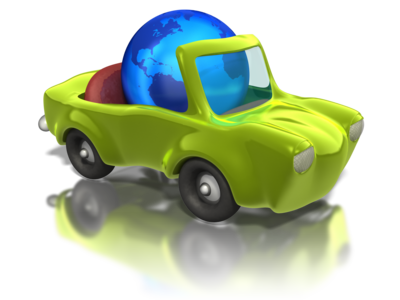
\includegraphics[height=0.3\textheight,keepaspectratio]{assets/car.png}
	\end{center}
		
	\pause
	
	\begin{conblock}{Mobilit\`{a} elettrica veicolare - CONTRO}
		\begin{itemize}
			\con {\large Tempi di ricarica Lunghi}
			\con {\large Durata Batterie limitata}
			\con {\large Posizione Colonnine}
		\end{itemize}
	\end{conblock}
	
\end{frame}

\begin{frame}
	\frametitle{Internet of Energy}
	\begin{problock}{Internet of Energy}
		\begin{itemize}
			\item {\large Infrastrutture}
			\item {\large Servizi}
		\end{itemize}	
	\end{problock}
	 
	\vspace*{1em}	 
	 
	\begin{center}
		
\includegraphics[height=0.3\textheight,keepaspectratio]{assets/ioe-logo.png}
	\end{center}
\end{frame}

\begin{frame}
	\frametitle{Architettura}
	\begin{problock}{Componenti}
		\begin{itemize}
			\item {\large Ontologia}
			\item {\large Semantic Informationn Broker}
			\item {\large Servizio Cittadino}
		\end{itemize}	
	\end{problock}
	
	\begin{center}
		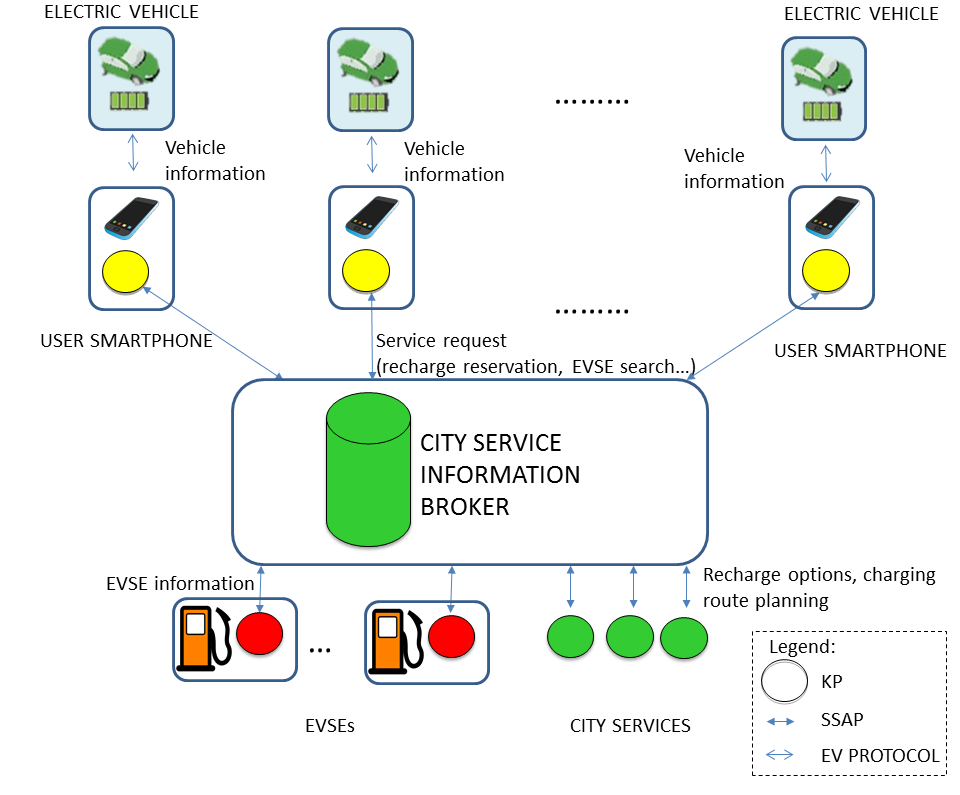
\includegraphics[height=0.65\textheight,keepaspectratio]{assets/architecture-without.png}
	\end{center}
\end{frame}

\begin{frame}
	\frametitle{Applicazione Mobile}
	\begin{problock}{Funzionalità}
		\begin{itemize}[<+->]
			\item {\large Interfaccia con Veicolo Reale}
			\item {\large Prenotazione Ricariche}
			\item {\large Profilo Altimetrico}
			\item {\large Consumo Energetico}
		\end{itemize}	
	\end{problock}
	
	\begin{center}
%		\includegraphics<1>[height=0.5\textheight,keepaspectratio]{assets/daily.png}

		\begin{tikzpicture}%[framed,background rectangle/.style={ultra thick,draw=white, top color=white, rounded corners}]
			\visible<1> {
				\node[inner sep=0pt] (daily) at (2,0)
	  				 {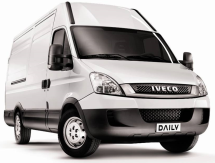
\includegraphics[width=.45\textwidth]{assets/daily.png}};
			}
			\visible<2> {
				\node[inner sep=0pt] (request) at (0,0)
	  				 {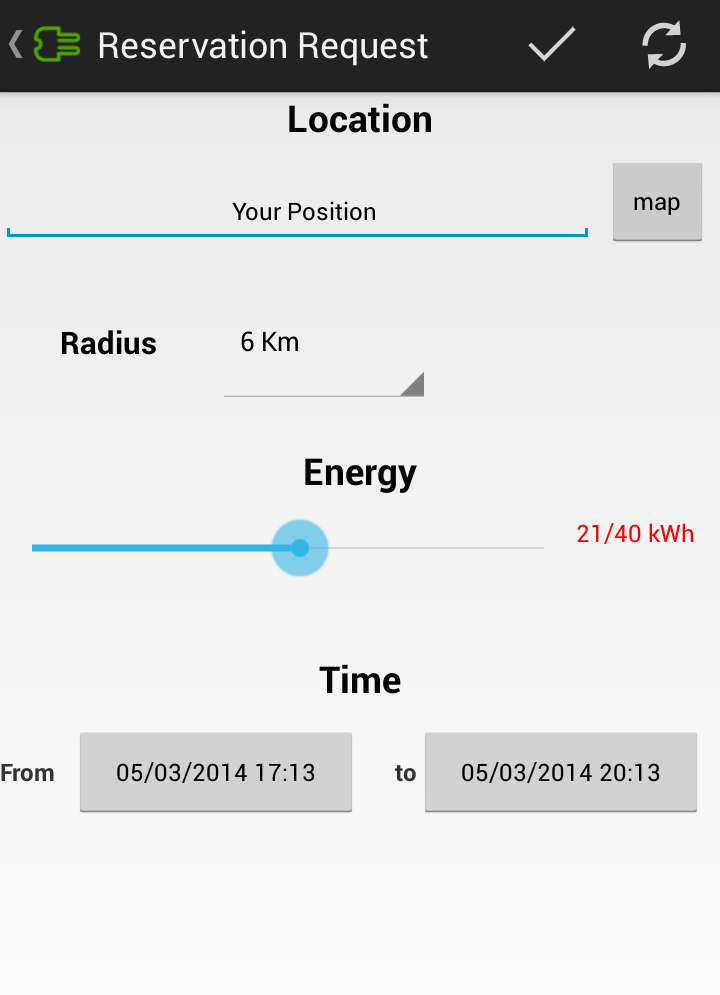
\includegraphics[width=.3\textwidth]{assets/mobile-app-charge-request.png}};
				\node[inner sep=0pt] (response) at (5,0)
	   				 {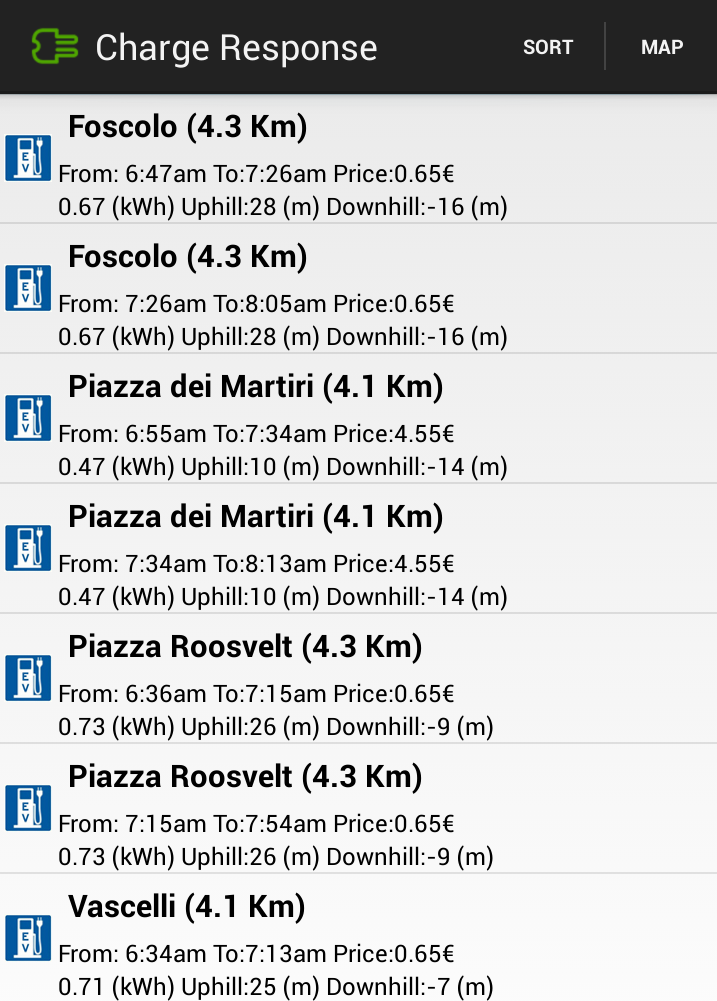
\includegraphics[width=.3\textwidth]{assets/mobile-app-charge-options.png}};
				\draw[->,thick] (request) -- (response) ;		
			}
			
			\visible<3> {
				\node[inner sep=0pt] (map) at (0,0)
	  				 {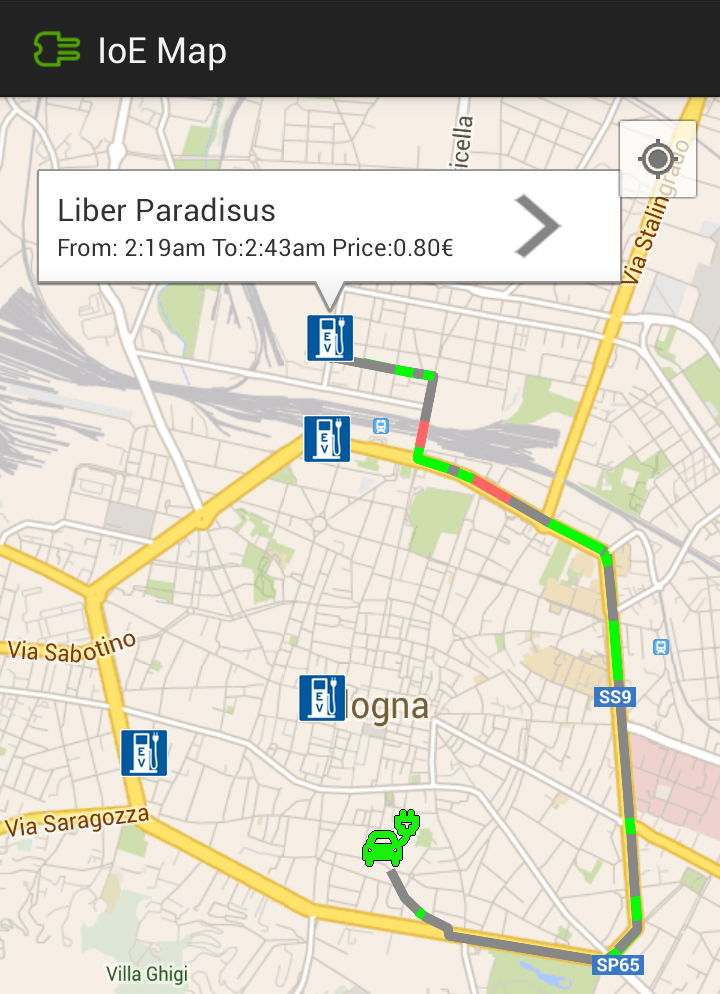
\includegraphics[width=.3\textwidth]{assets/mobile-app-map.png}};
				\node[inner sep=0pt] (graph) at (5,0)
	   				 {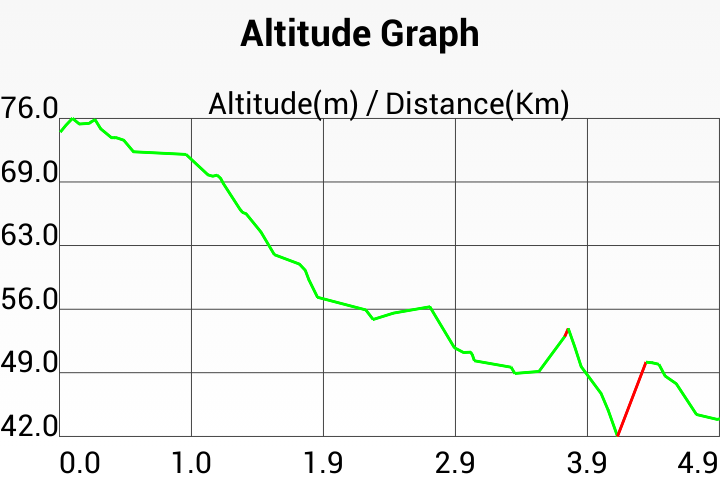
\includegraphics[width=.5\textwidth]{assets/mobile-app-alti-graph.png}};	
			}
			
			\visible<4> {
				\node[inner sep=0pt] (request) at (0,0)
	  				 {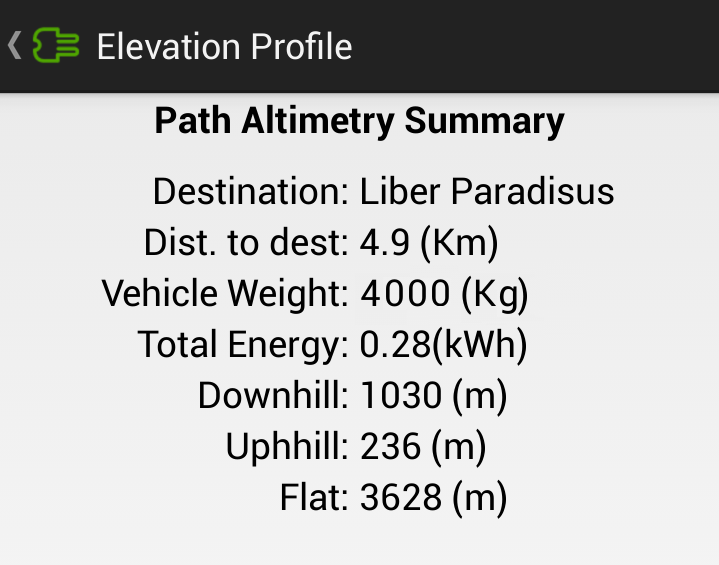
\includegraphics[width=.43\textwidth]{assets/mobile-app-altimetry-summary.png}};
				\node[inner sep=0pt] (response) at (5,0)
	   				 {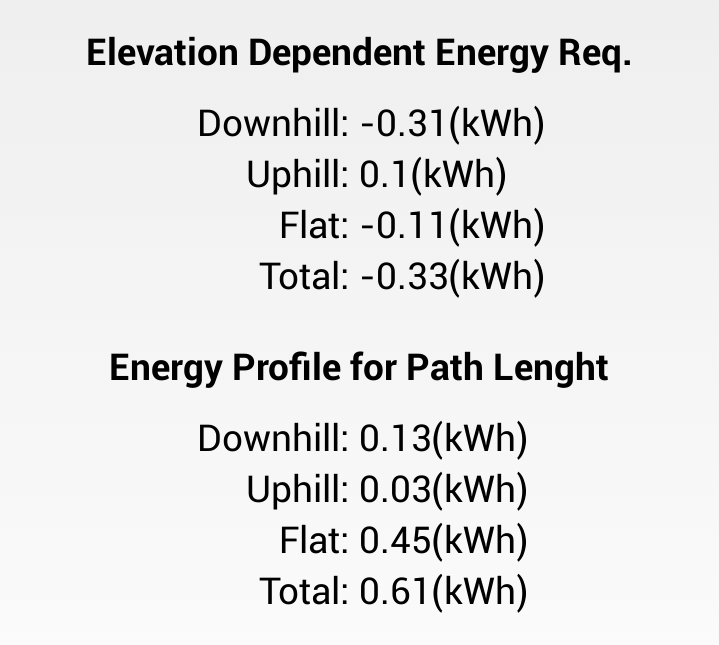
\includegraphics[width=.4\textwidth]{assets/mobile-app-energy.png}};	
			}
		\end{tikzpicture}
	\end{center}
\end{frame}

\begin{frame}
	\frametitle{Simulatore}
	\begin{problock}{Architettura}
		\begin{itemize}[<+->]
			\item {\large SUMO}
			\item {\large OMNeT++}
			\item {\large Veins}
		\end{itemize}	
	\end{problock}
	
	\begin{center}
		\includegraphics<1>[height=0.5\textheight,keepaspectratio]{assets/sumo.jpg}
		\includegraphics<2>[height=0.5\textheight,keepaspectratio]{assets/sumo-2.jpg}
		\includegraphics<3>[height=0.5\textheight,keepaspectratio]{assets/veins-arch.png}
	\end{center}
	
\end{frame}

\begin{frame}
	\frametitle{Simulatore}
	\begin{problock}{Dati Studiabili}
		\begin{itemize}[<+->]
			\item {\large Occupazione Colonnine}
			\item {\large Comportamento veicoli}
			\item {\large Richieste fallite}
			\item {\large Consumo batteria}
		\end{itemize}	
	\end{problock}
	
	\begin{center}
		\includegraphics<1>[width=0.7\textwidth,keepaspectratio]{assets/anxiety30-occupation.eps}
		\includegraphics<2>[width=0.7\textwidth,keepaspectratio]{assets/anxiety30-states.eps}
		\includegraphics<3>[width=0.7\textwidth,keepaspectratio]{assets/anxiety30-vapo.eps}
		\includegraphics<4>[width=0.45\textwidth,keepaspectratio]{assets/mdn-consumo.png}
		\hspace{1em}
		\includegraphics<4>[width=0.45\textwidth,keepaspectratio]{assets/mdn-consumo-pendenza.png}
	\end{center}
		
\end{frame}

\end{document}